\documentclass{standalone}
\usepackage{tikz}
\usetikzlibrary{patterns, positioning}
\usepackage[sfdefault]{ClearSans} %% option 'sfdefault' activates Clear Sans as the default text font
\usepackage[T1]{fontenc}

\begin{document}
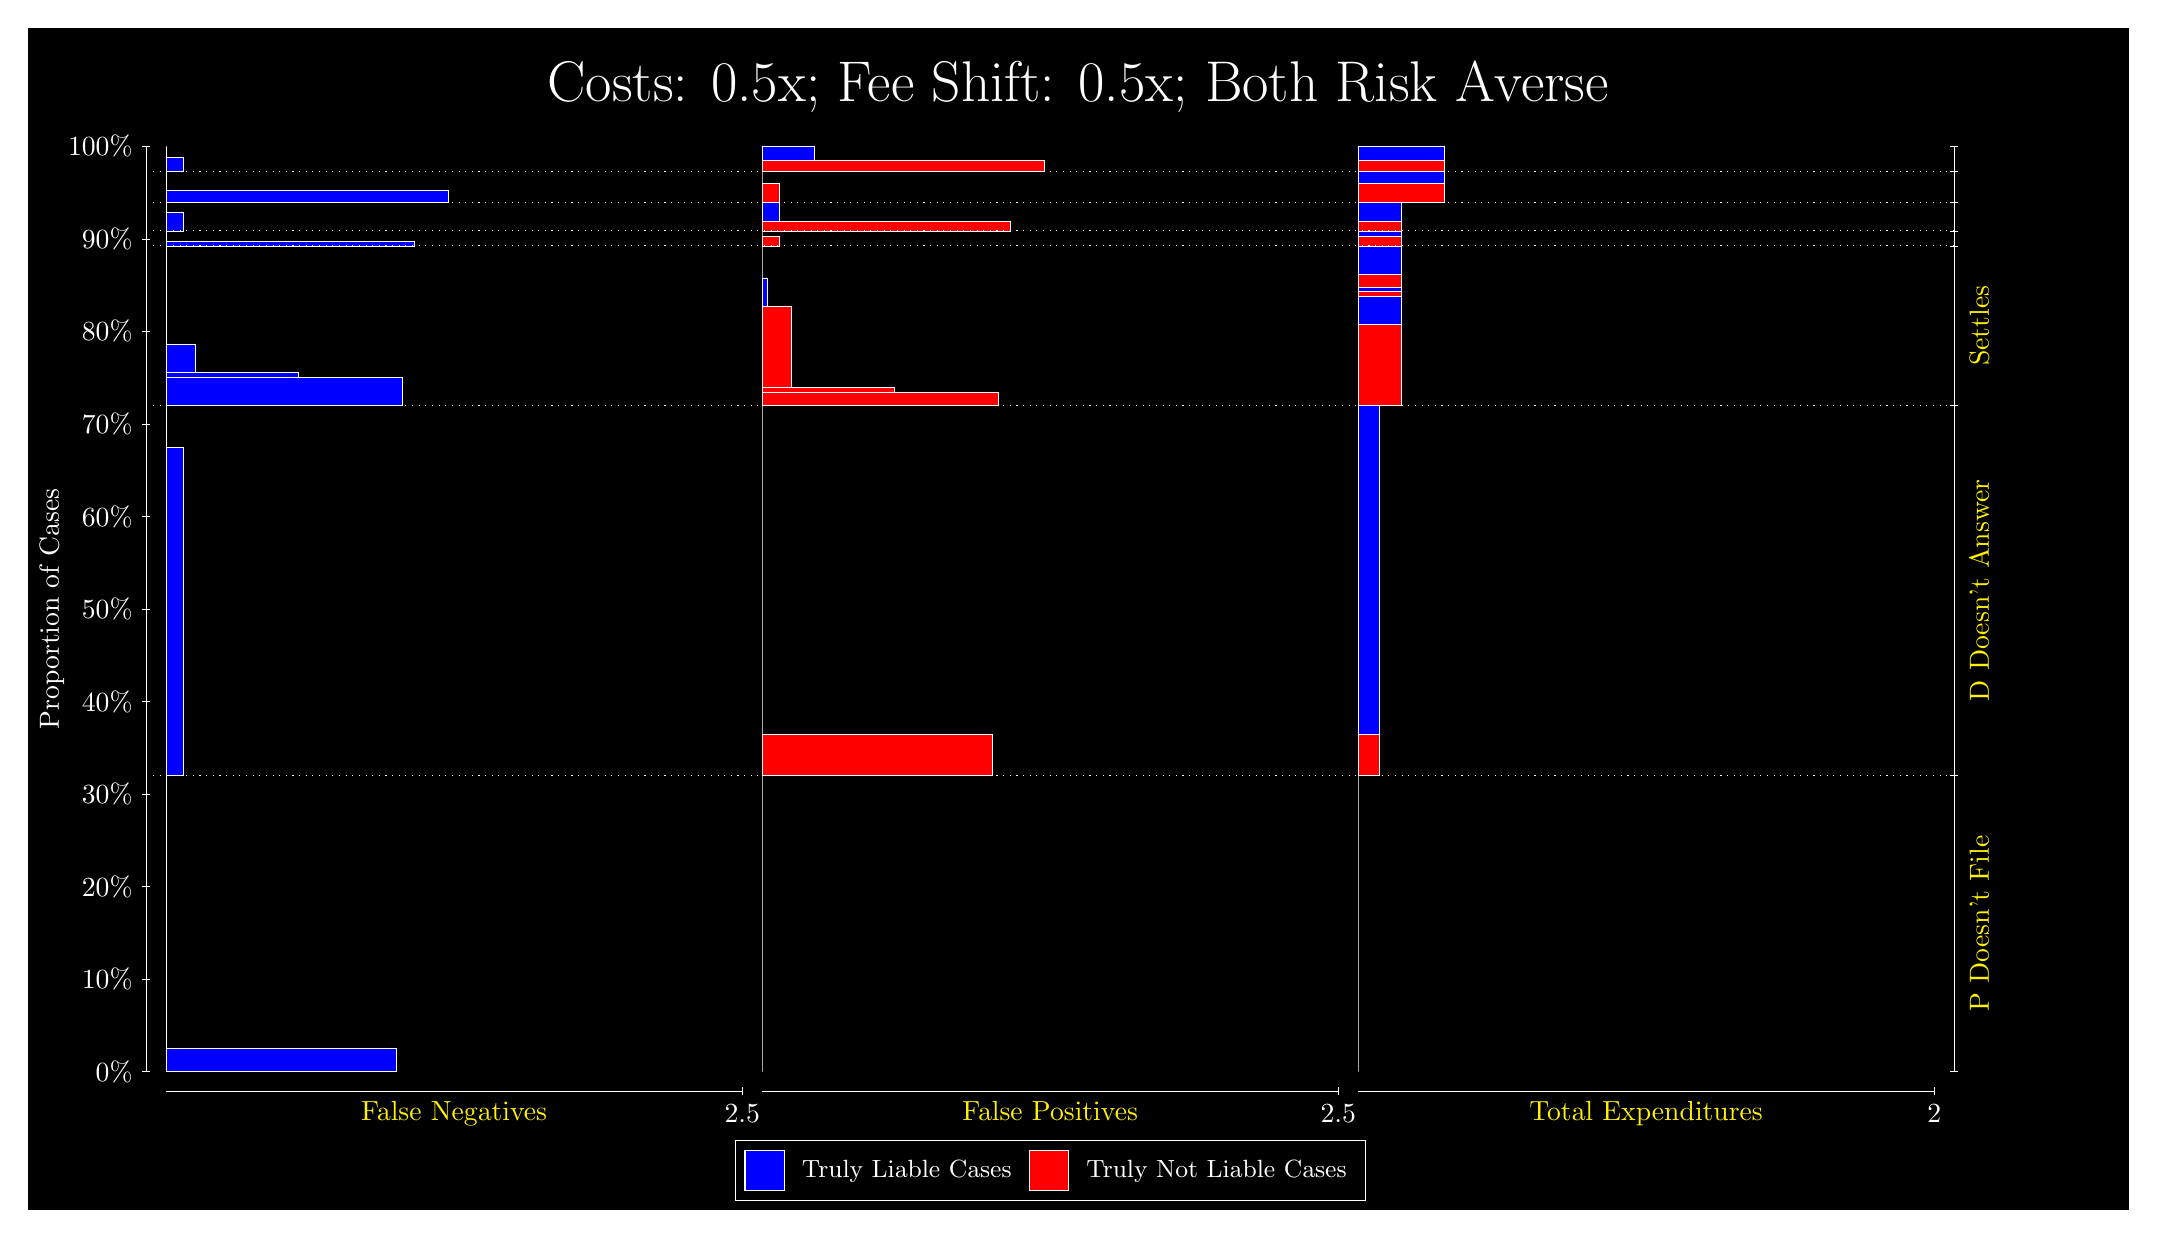
\begin{tikzpicture}
\draw[fill=black] (0,0) rectangle (26.667,15);
\draw[text=white] (0,13.5) rectangle (26.667,15) node[midway] {\huge Costs: 0.5x; Fee Shift: 0.5x; Both Risk Averse};
\draw[white, very thin] (1.5,1.75) -- (1.5,13.5);
\node[rotate=90, text=white, anchor=center] at (0.3, 7.625) {Proportion of Cases};
\draw[white, very thin] (1.45,1.75) -- (1.55,1.75);
\node[text=white, anchor=east] at (1.45, 1.75) {0\%};
\draw[white, very thin] (1.45,2.925) -- (1.55,2.925);
\node[text=white, anchor=east] at (1.45, 2.925) {10\%};
\draw[white, very thin] (1.45,4.1) -- (1.55,4.1);
\node[text=white, anchor=east] at (1.45, 4.1) {20\%};
\draw[white, very thin] (1.45,5.275) -- (1.55,5.275);
\node[text=white, anchor=east] at (1.45, 5.275) {30\%};
\draw[white, very thin] (1.45,6.45) -- (1.55,6.45);
\node[text=white, anchor=east] at (1.45, 6.45) {40\%};
\draw[white, very thin] (1.45,7.625) -- (1.55,7.625);
\node[text=white, anchor=east] at (1.45, 7.625) {50\%};
\draw[white, very thin] (1.45,8.8) -- (1.55,8.8);
\node[text=white, anchor=east] at (1.45, 8.8) {60\%};
\draw[white, very thin] (1.45,9.975) -- (1.55,9.975);
\node[text=white, anchor=east] at (1.45, 9.975) {70\%};
\draw[white, very thin] (1.45,11.15) -- (1.55,11.15);
\node[text=white, anchor=east] at (1.45, 11.15) {80\%};
\draw[white, very thin] (1.45,12.325) -- (1.55,12.325);
\node[text=white, anchor=east] at (1.45, 12.325) {90\%};
\draw[white, very thin] (1.45,13.5) -- (1.55,13.5);
\node[text=white, anchor=east] at (1.45, 13.5) {100\%};

\draw[white, very thin] (24.457,1.75) -- (24.457,13.5);
\draw[white, very thin] (24.407,1.75) -- (24.507,1.75);
\node[anchor=west] at (24.407, 1.75) {};
\draw[white, very thin] (24.407,5.5119) -- (24.507,5.5119);
\node[anchor=west] at (24.407, 5.5119) {};
\draw[white, very thin] (24.407,10.209) -- (24.507,10.209);
\node[anchor=west] at (24.407, 10.209) {};
\draw[white, very thin] (24.407,12.235) -- (24.507,12.235);
\node[anchor=west] at (24.407, 12.235) {};
\draw[white, very thin] (24.407,12.427) -- (24.507,12.427);
\node[anchor=west] at (24.407, 12.427) {};
\draw[white, very thin] (24.407,12.79) -- (24.507,12.79);
\node[anchor=west] at (24.407, 12.79) {};
\draw[white, very thin] (24.407,13.184) -- (24.507,13.184);
\node[anchor=west] at (24.407, 13.184) {};
\draw[white, very thin] (24.407,13.5) -- (24.507,13.5);
\node[anchor=west] at (24.407, 13.5) {};

\draw[white, very thin, fill=blue] (1.75,1.75) rectangle (4.6775,2.0499);
\draw[white, very thin, fill=red] (1.75,2.0499) rectangle (1.75,5.5119);
\draw[white, very thin, fill=blue] (1.75,5.5119) rectangle (1.9696,9.6831);
\draw[white, very thin, fill=red] (1.75,9.6831) rectangle (1.75,10.209);
\draw[white, very thin, fill=blue] (1.75,10.209) rectangle (4.7507,10.569);
\draw[white, very thin, fill=blue] (1.75,10.569) rectangle (3.4333,10.626);
\draw[white, very thin, fill=blue] (1.75,10.626) rectangle (2.1159,10.98);
\draw[white, very thin, fill=red] (1.75,10.98) rectangle (1.75,12.235);
\draw[white, very thin, fill=blue] (1.75,12.235) rectangle (4.8971,12.3);
\draw[white, very thin, fill=red] (1.75,12.3) rectangle (1.75,12.427);
\draw[white, very thin, fill=blue] (1.75,12.427) rectangle (1.9696,12.665);
\draw[white, very thin, fill=red] (1.75,12.665) rectangle (1.75,12.79);
\draw[white, very thin, fill=blue] (1.75,12.79) rectangle (5.3362,12.937);
\draw[white, very thin, fill=red] (1.75,12.937) rectangle (1.75,13.184);
\draw[white, very thin, fill=blue] (1.75,13.184) rectangle (1.9696,13.367);
\draw[white, very thin, fill=red] (1.75,13.367) rectangle (1.75,13.5);
\draw[white, very thin, fill=red] (9.3189,1.75) rectangle (9.3189,5.2119);
\draw[white, very thin, fill=blue] (9.3189,5.2119) rectangle (9.3189,5.5119);
\draw[white, very thin, fill=red] (9.3189,5.5119) rectangle (12.246,6.0379);
\draw[white, very thin, fill=blue] (9.3189,6.0379) rectangle (9.3189,10.209);
\draw[white, very thin, fill=red] (9.3189,10.209) rectangle (12.32,10.374);
\draw[white, very thin, fill=red] (9.3189,10.374) rectangle (11.002,10.44);
\draw[white, very thin, fill=red] (9.3189,10.44) rectangle (9.6848,11.465);
\draw[white, very thin, fill=blue] (9.3189,11.465) rectangle (9.3921,11.819);
\draw[white, very thin, fill=blue] (9.3189,11.819) rectangle (9.3189,12.235);
\draw[white, very thin, fill=red] (9.3189,12.235) rectangle (9.5384,12.362);
\draw[white, very thin, fill=blue] (9.3189,12.362) rectangle (9.3189,12.427);
\draw[white, very thin, fill=red] (9.3189,12.427) rectangle (12.466,12.552);
\draw[white, very thin, fill=blue] (9.3189,12.552) rectangle (9.5384,12.79);
\draw[white, very thin, fill=red] (9.3189,12.79) rectangle (9.5384,13.037);
\draw[white, very thin, fill=blue] (9.3189,13.037) rectangle (9.3189,13.184);
\draw[white, very thin, fill=red] (9.3189,13.184) rectangle (12.905,13.317);
\draw[white, very thin, fill=blue] (9.3189,13.317) rectangle (9.9776,13.5);
\draw[white, very thin, fill=red] (16.888,1.75) rectangle (16.888,5.2119);
\draw[white, very thin, fill=blue] (16.888,5.2119) rectangle (16.888,5.5119);
\draw[white, very thin, fill=red] (16.888,5.5119) rectangle (17.162,6.0379);
\draw[white, very thin, fill=blue] (16.888,6.0379) rectangle (17.162,10.209);
\draw[white, very thin, fill=red] (16.888,10.209) rectangle (17.437,11.234);
\draw[white, very thin, fill=blue] (16.888,11.234) rectangle (17.437,11.594);
\draw[white, very thin, fill=red] (16.888,11.594) rectangle (17.437,11.66);
\draw[white, very thin, fill=blue] (16.888,11.66) rectangle (17.437,11.716);
\draw[white, very thin, fill=red] (16.888,11.716) rectangle (17.437,11.881);
\draw[white, very thin, fill=blue] (16.888,11.881) rectangle (17.437,12.235);
\draw[white, very thin, fill=red] (16.888,12.235) rectangle (17.437,12.362);
\draw[white, very thin, fill=blue] (16.888,12.362) rectangle (17.437,12.427);
\draw[white, very thin, fill=red] (16.888,12.427) rectangle (17.437,12.552);
\draw[white, very thin, fill=blue] (16.888,12.552) rectangle (17.437,12.79);
\draw[white, very thin, fill=red] (16.888,12.79) rectangle (17.986,13.037);
\draw[white, very thin, fill=blue] (16.888,13.037) rectangle (17.986,13.184);
\draw[white, very thin, fill=red] (16.888,13.184) rectangle (17.986,13.317);
\draw[white, very thin, fill=blue] (16.888,13.317) rectangle (17.986,13.5);
\draw[white, dotted] (1.5,5.5119) -- (24.457,5.5119);
\draw[white, dotted] (1.5,10.209) -- (24.457,10.209);
\draw[white, dotted] (1.5,12.235) -- (24.457,12.235);
\draw[white, dotted] (1.5,12.427) -- (24.457,12.427);
\draw[white, dotted] (1.5,12.79) -- (24.457,12.79);
\draw[white, dotted] (1.5,13.184) -- (24.457,13.184);
\draw[white, very thin] (1.75,1.5) -- (9.0689,1.5);
\node[text=yellow, anchor=north] at (5.4094, 1.5) {False Negatives};
\draw[white, very thin] (9.0689,1.45) -- (9.0689,1.55);
\node[text=white, anchor=north] at (9.0689, 1.45) {2.5};

\draw[white, very thin] (9.3189,1.5) -- (16.638,1.5);
\node[text=yellow, anchor=north] at (12.978, 1.5) {False Positives};
\draw[white, very thin] (16.638,1.45) -- (16.638,1.55);
\node[text=white, anchor=north] at (16.638, 1.45) {2.5};

\draw[white, very thin] (16.888,1.5) -- (24.207,1.5);
\node[text=yellow, anchor=north] at (20.547, 1.5) {Total Expenditures};
\draw[white, very thin] (24.207,1.45) -- (24.207,1.55);
\node[text=white, anchor=north] at (24.207, 1.45) {2};

\node[text=yellow, centered, rotate=90] at (24.777, 3.6309) {P Doesn't File};
\node[text=yellow, centered, rotate=90] at (24.777, 7.8605) {D Doesn't Answer};
\node[text=yellow, centered, rotate=90] at (24.777, 11.222) {Settles};





\draw (12.978300999999998,1.5) node[draw=none] (baseCoordinate) {};
\begin{scope}[align=center]
        \matrix[scale=0.5, draw=white, below=0.5cm of baseCoordinate, nodes={draw}, column sep=0.1cm]{
            \node[rectangle, draw, minimum width=0.5cm, minimum height=0.5cm, fill=blue] {}; &
            \node[draw=none, font=\small, text=white] (B) {Truly Liable Cases}; &
            \node[rectangle, draw, minimum width=0.5cm, minimum height=0.5cm, fill=red] {}; &
            \node[draw=none, font=\small, text=white] (B) {Truly Not Liable Cases}; \\
            };
\end{scope}

\end{tikzpicture}
\end{document}